\section{Efficiency corrections}
%I need to go back and improve the writing and justification here
	As was discussed in section \ref{jet_toy_model}, the selection of a jet cone limits the accuracy of the energy correlator calculation in a way that depends on $R_L$. 
	Beyond the problems noted in that model, one also has the issue of normalization and efficiency. 
	Any set of pairs (or triplets or N-point combinations) measured in a calorimeter needs to be corrected for the overabundance of pairs sitting at the discretized lattice in $R_L$. 
	To proceed with the efficiency correction on the two point correlator, one must begin with considering the continuous case. 
	Any jet cone limits the number of identified pairs which has the potential to bias the results, thus an efficiency of identification of contained pairs must be introduced.
	Begin by drawing a jet cone of radius $R_j$ in the $\eta-\varphi$ plane of some idealized zero-width tower calorimeter, and select some point in the jet offset from the center by some distance $\mathscr{r}$ and angle $\lambda$, then draw another circle of radius $R_L$ around this point limited to the jet cone--representing all pairs to the chosen point that lie within the jet--as show in fig \ref{fig:eff_corr}. Then the efficiency ratio defined as geometric pairs in jet over geometric pairs in the phase space gives
	\begin{equation}
		\begin{split}
			\tilde{\varepsilon} \left( R_L , R_J \right) 	&= \frac{\int_{0}^{2 \pi} \dd \lambda \int_{\textrm{max}\left\{0,R_{L}-R_j\right\}}^{R_{j}} \dd \mathcal{r} C_{inc}}{C_{Total}} \\
									&= \frac{\int_{0}^{2 \pi} \dd \lambda \int_{\textrm{max}\left\{0, R_L-R_j \right\} }^{R_j} \dd \mathcal{r} 2\int_{0}^{\theta_f} \dd \theta \pi \theta R_L}{\int_{0}^{2 \pi} \dd \lambda \int_{0}^{R_j} \dd \mathcal{r} 2 \pi R_L}
		\end{split}
		\label{eq:eff_cont_set}
	\end{equation}
	Where $\theta$ is the polar angle measured around the circle of pairs, $C_{inc}$ is the circumference of the circles of pairs, $C_{Total}$  is just the total pairs in the phase space and is used as a normalization factor to allow for comparisons with the discretized case.
	The bounds for the $\theta$ integral reflect that two points are symmetric around the axis defined by the centers of the two circles, and $\cos \theta_f = \frac{R_L^2 + \mathcal{r}^2 - R_j^2}{2 \mathcal{r} R_j^2}$, 
	and the bounds on $\mathcal{r}$ are given to keep at least one pair within the jet in the numerator. 
	Switching the order of integration in eq (\ref{eq:eff_cont_set}) and bounds allows for a version of this integral to be done, and then the resulting elliptical integral is evaluated around $\textrm{arccos}\left( \frac{R_L}{2R_j} \right)$ for an approximate answer 
	\begin{equation}
		\begin{split}
			\tilde{\varepsilon} \left( R_L, R_j \right) 	&= \frac{R_L}{2 \pi R_j^2} \sqrt{4 R_j^2 - R_L^2} + \frac{E \left( \textrm{arccos} \left( \frac{R_L}{2R_J} \right) \left| \frac{R_L^2}{R_j^2} \right. \right)}{2\pi} \\
									& \approx \sqrt{R_L}{2 \pi R_j^2} \left[ \frac{4 R_j^2 - R_L^2} %hey numbskull, what goes here?????
									+ R_j \textrm{arccos} \left( \frac{R_L}{2 R_J} \right) \right. \\ & \left. \hspace{1 cm}- \frac{R_L}{3} \left( \textrm{arccos} \left(\frac{R_L}{2R_J} \right) \right)^3 + \mathcal{O}\left( \left[\textrm{arccos} \left(\frac{R_L}{2R_J} \right) \right]^5 \right) \right]
		\end{split}
		\label{eq:eff_cont}
	\end{equation}
	
	\hspace{0.5 cm} Switching to the discretized case, one introduces the new parameters $\delta, \gamma$ being the size of a calorimeter tower in $\varphi, \eta$ respectively. First take $\delta \approx \gamma$ such that the problem is one of square towers, which, for the purposes of analysis of sPHENIX data is appropriate, given that the towers of each calorimeter are almost square--see sections \ref{sect:HCAL_cons} and \ref{sect:EMCAL_cons}. 
	Then, we start with a definition of the circumference to use in this case. 
	One states that all towers can be expressed as a set of points of the form $(p \delta , q \delta)$ s.t. $p, q \in \mathbb{Z}$, and the equivalent measure to the circumference of the continuous around a central point $P_c=(p_c, q_c)\delta$ can be stated as 
	\begin{equation}
		\left|\mathcal{C}\left[R_L, \delta,\left(p_c, q_c\right)\right]\right| = \left| \left\{ P | \left(p - p_c\right)^2 + \left(q-q_c\right)^2 = \frac{R_L^2}{\delta^2} \right\}\right|
		\label{eq:N_pairs_disc}
	\end{equation}
	A natural extension from this measure tells us that $\frac{R_L^2}{\delta^2} = \mathbb{Z}$ which gives a natural binning for the energy-energy correlator, if plotted as a function of $R_L^2$. 
	From here, the equivalent expression to eq. \ref{eq:eff_cont_set} can be stated as 
	\begin{equation}
		\begin{split}
			\tilde{\varepsilon} \left(R_L, R_j, \delta \right) &= \frac{ \sum_{(m,n) \in \textrm{Disk}\left(R_j\right)} \left| \mathcal{C} \left[R_L, \delta \left( m, n\right)\right] \cap \textrm{Disk} \left( R_j \right) \right|}{\left| \textrm{Disk}\left(R_j\right)\right| \left|\mathcal{C}\left[R_L, \delta,\left(0, 0\right)\right]\right|}
		\end{split}
		\label{eq:eff_disc_set}
	\end{equation}
	where Disk$\left(R_j\right)$ is the collection of points that lie within a circle of radius $R_j$ and $\mathcal{C}$ is the collection of points at exactly $R_L$ from the center point $(m,n)\delta$. 
	The cardinality of these sets can be found by noting that $|\mathcal{C}|$ is simply the sum-of-squares function $r_2\left( \frac{R_L^2}{\delta^2} \right)$ and $\left| \textrm{Disk}\left(R_j\right)\right|$ is Gauss's Circle Problem \cite{Hilbert2021}. 

	In order to solve for the numerator, one takes a second disk of radius $R'_j$ such that, 
	\begin{equation}
		\mathcal{C} \left[R_L, \delta \left( m, n\right) \cap \textrm{Disk}\left( R'_j \right) \right] = \mathcal{C} \hspace{0.5 cm} \forall (m,n ) \in \textrm{Disk}\left(R_j\right)
		\label{eq:larger_set}
	\end{equation}
	Which, allows for the folding of the summation into a problem of set theory, noting that 
	\begin{equation}
		\begin{split}
			\textrm{Disk}\left(R'_j\right) &=  \textrm{Disk}\left(R_j\right) \cup \sum_{(m,n)} \mathcal{C} \\
			\Rightarrow |\textrm{Disk}\left(R_j \right) \cap \sum_{(m,n)} \mathcal{C}| &= \left| \textrm{Disk}\left(R_j\right) \right| + \left| \sum_{(m,n)} \mathcal{C} \right| - \left| \textrm{Disk}\left(R'_j\right) \right| \\
			&= \left| \textrm{Disk}\left(R_j\right)\right| \left( 1+ \left|\mathcal{C}\left[R_L, \delta,\left(0, 0\right) \right] \right| \right) - \left| \textrm{Disk}\left(R'_j\right)\right| \\
		\end{split}
		\label{eq:set_card}
	\end{equation}
	Setting $R'_j = R_j + R_L$ as the largest value for $R'_j$ which corresponds to a collection of pairs centered on one of the edges of the faces, the equivalent to eq \ref{eq:eff_cont} is simply 
	\begin{equation}
		\tilde{\varepsilon}\left( R_L, R_j, \delta \right) = 1 - \frac{1}{r_2 \left( \frac{R_L^2}{\delta^2} \right)} \left[ \left. \sum^{\frac{\left(R_j + R_L \right)^2}{\delta^2}i}_{i=\frac{R_j^2}{\delta^2}} r_2(i) \right/ \sum^{\frac{R_j^2}{\delta^2}i}_{i=0} r_2(i) \right]
		\label{eq:eff_disc}
	\end{equation}
	To approximate the solution one can the identity from Hardy and Ramanujan \cite{Chan2019}, however, for our purposes, it suffices to use numerical solutions for the special cases that are relevant to the detector as is shown in fig \ref{fig:eff_corr}
	\begin{figure}
		\begin{center}
			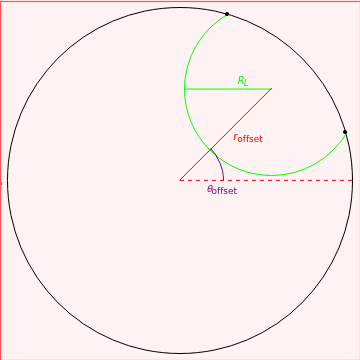
\includegraphics{img/continuous_pair_corrections}
			\caption{The continuous and discretized calorimeters for phase space and discretization efficiency correction to smooth distribution and reduce bin width selection dependence}
		\end{center}
		\label{fig:eff_corr}
	\end{figure}
	Thus, the full efficiency correction on $\Delta R_L$ to correct for both edge effects of the jet cone and the effects of a finite spatial resolution on the calorimeters is 
	\begin{equation}
		\begin{split}
			\varepsilon \left( R_L, R_j, \delta \right) &= \frac{R_L r_2 \left( \frac{R_L^2}{\delta^2} \right)}{2 \pi R_j^2 } \left[  \frac{\sqrt{4 R_j^2 -R_L^2} + R_j E \left( \textrm{arccos} \left( \frac{R_L}{2R_J} \right) \left| \frac{R_L^2}{R_j^2} \right. \right) } {r_2 \left( \frac{R_L^2}{\delta^2} \right) -  \left. \sum^{\frac{\left(R_j + R_L \right)^2}{\delta^2}i}_{i=\frac{R_j^2}{\delta^2}} r_2(i) \right/ \sum^{\frac{R_j^2}{\delta^2}i}_{i=0} r_2(i) }  \right]
		\end{split}
	\end{equation}
\section{Uncertainties}
	\subsection{Statistical Uncertianity}

	\subsection{Systematic Uncertianity sources}
	\subsection{Binning Uncertianity}
	\subsection{Systematic Uncertainties}
